\subsection{The Server}
To construct the main sever, we chose java\cite{java} as our
programming language because of its multi platform abilities and the development
suit of eclipse\cite{eclipse} called swt\cite{swt} as our window-builder framework. We only used basic java libraries which came by default
with the eclipse IDE\cite{ide} environment, namely the
jdk7-openjdk\cite{open_jdk} package. 

When the Panstamp server is connected to the Java server, the latter takes the data given by the Panstamp server thanks to the RxTx library \cite{rxtx} and passes the information to the parser for processing. 

The server checks with an external timed thread the state of each known device.
This thread checks the current state of the device and, if necessary, sets the
state back to standby if too much time since the last change has passed. Therefore,
the thread compares the timestamp of the last state change with the current
time. Furthermore, it checks if the neighbor module is still detected by the device or not.

\begin{figure*}[ht]
	\centerline{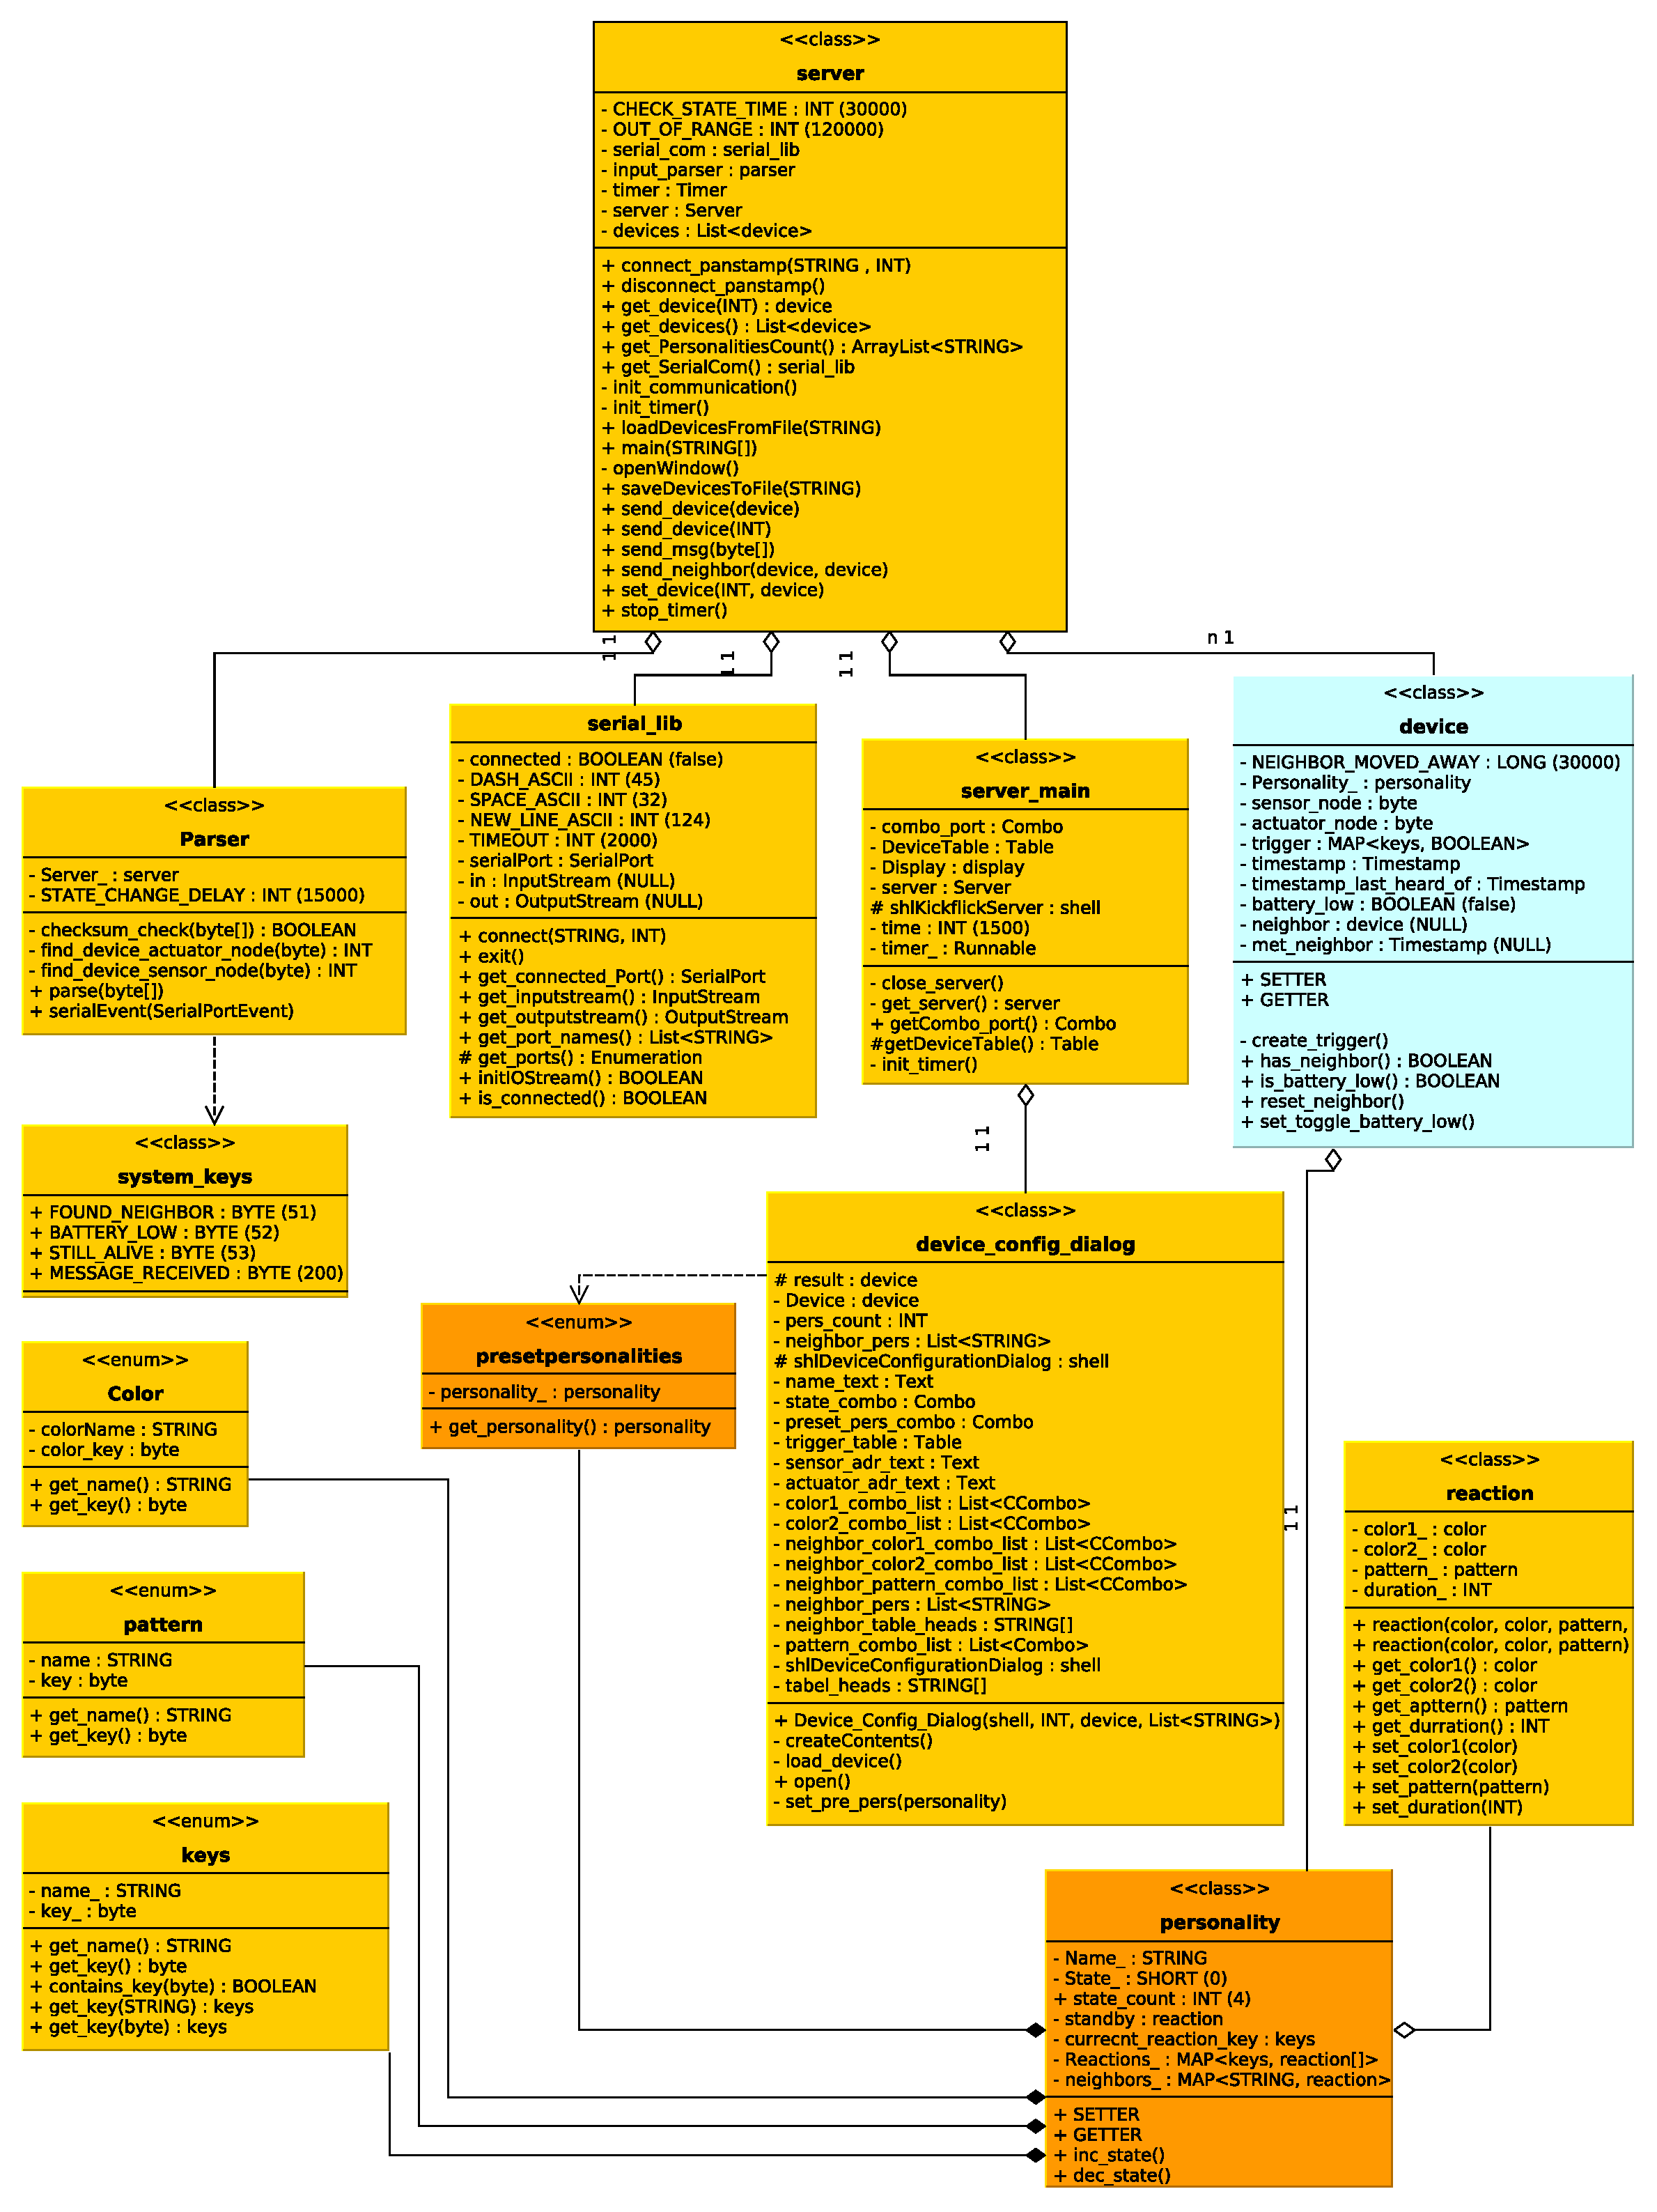
\includegraphics[width=\textwidth]{./graph/general.pdf}}
	\caption{UML Diagram of the Server Structure}
	\label{fig:server_uml}
\end{figure*}


\subsubsection{Panstamp-to-Java server message}
\label{sec:Panstamp-to-Java server message}
All messages sent by the Panstamp server to the Java Server contain four bytes. The message's length was set to a single value to achieve a better communication work-flow and to limit the communication's traffic to a minimum. Table~\ref{Panstamp-to-Java} shows the general structure of a message.


\begin{table}[h]
  \centering
  \begin{tabular}{ c | c | c | c }
    \hline
    \textbf{Byte 1} & \textbf{Byte 2} & \textbf{Byte 3} & \textbf{Byte 4} \\ [0.5ex]    
    \hline
    Sender's & Admin & Neighbor's Id| & Checksum  \\
    Id & Key & Dummy & \\
    \hline
  \end{tabular}
  \caption[Pamstamp-to-Java]%
          {Panstamp-to-Java server message's structure}
  \label{Panstamp-to-Java}
\end{table}

\begin{itemize}
\item \textbf{Sender's Id} is the Id of the network node that wants to report an event
\item \textbf{Admin Key} indicates the event reported by the entity. See table~\ref{Admin Keys} for further information.
\item \textbf {Neighbor's Id | Dummy } When the Admin Key equals NEARNODEEVENT, this byte contains the Id of the found neighbor node. For other keys this byte is ignored
\item \textbf {Checksum} This byte is the sum of bytes 1, 2 and 3 (modulo 256)
\end{itemize}

Table~\ref{Admin Keys} displays all the possible Admin Keys:

\begin{table}[h]
  \centering
  \begin{tabular}{ c | c }
    \hline
    \textbf{Name} & \textbf{Value}\\ [0.5ex]    
    \hline
    Shake Event & 31 \\
    Kick Event  & 32 \\
    Near Node Event & 51\\
    Low battery & 52\\
    In Range & 53\\   
    \hline
  \end{tabular}
  \caption[Admin Keys]%
          {Admin Keys}
  \label{Admin Keys}
\end{table}

\begin{itemize}
\item \textbf {Shake Event} indicates the entity has been shaken slightly so it is swaying
\item \textbf {Kick Event} means that the entity has been kicked or moved with a strong blow
\item \textbf {Near Node Event} signifies the entity has detected another entity which is really close to it
\item \textbf {Low Battery} warns the server that the entity's battery has to be recharged as soon as possible
\item \textbf {In range} indicates the server that the entity is still in range
\end{itemize}




\subsubsection{The Parser}
 
First, the parser checks whether the length of the package is exactly four bytes
and if the last byte, which is supposed to be a checksum summing the byte values
of every other bytes in the message, matches the checksum calculated by the
server. If everything is correct, the parser then searches for a known device in
the modules' list of the server. If it doesn't find a match, the parser will create a new device
with default settings. 

Once a device was found or created, the parser begins to compare the second byte of the message with the admin keys stored in the server data (see table~\ref{Admin Keys} ). For example, if the received message contains the number''52'' in its second byte, the parser will then recognize this as the ''the battery is low'' key and will toggle the boolean value battery\_low of the device to true. 

The keys 'Shake Event', 'Kick Event' and 'Near Node Event' can be ignored by a module if in its settings those events are disabled. In the Configuration Dialog Window, in the 'basic' tab, the user can activate or disable the effect each of those three keys produces in a specific device. 
Therefore, when a message with one of these keys is received, the parser checks the configured settings of the corresponding device and verifies if the key should be attended to or ignored. 
 
When enabled, the keys 'Shake event' and 'Kick Event' change the module's state to the next stage and led pattern data (pattern and 2 colors) that corresponds to the new module's state will be sent to the server-panStamp using the RxTx-library. 

When activated, the 'Near Node Event' key changes the led patterns of the two involved modules (a module and the neighbour it detected). For this, the Java server has to sent two messages (for the two devices) with the same led pattern data to the server-panstamp.  

No matter if a correct message leads to a state change or not, the device's timestamp will be updated to the time of the last correct received message. If the module's state did change, the server also stores another timestamp that reflects the time when the last state change happened.

\subsubsection{Device and Personality Structure}
The device class contains an instance of the personality class and the server class holds a list of all known devices.

Devices can be seen as a representation of the hardware modules with the two panStamps in them. It refers to the hardware and for this reason stores the Id's of the panStamps. Additionally, this class stores a first timestamp of the last received message from a module, a second timestamp of the last module's state change and a third timestamp of the last 'near neighbor' event. These data is accessible through ''get'' functions as well as mostly modifiable through ''set'' functions.

The personality class stores the reaction of a particular device depending on the admin keys, neighbors and the state of the device. To implement the set of possible reactions, this class stores a map of reactions (an array of instances of the class 'reaction') with the corresponding activator keys (instances of the enumeration 'keys').

For instance, if the parser receives a message, the reaction map will be searched for the key given by the message. If the key exists in the map, the reaction array will be returned and the personality returns the proper reaction that fits the current state. If the map holds no entry for that key, the reaction map returns a default reaction array.

The possible reactions for each detected neighbor are also stored in a map. This
map contains the name of the neighbour' personality and its the corresponding reaction (when this neighbour is found). 

Reactions in a device are represented by a class called reaction. This class stores information
about colors, patterns and the duration of each reaction (for how long time the reaction will be visible).

To get the server and the project running without setting up every single device
by hand, a enumeration for pre defined personalities was created. One can select
between each of those personalities. Once a pre defined personality is selected,
the previous personality of the current device will be overwritten. It is also possible to save the current devices to a file so that they can be loaded again after restarting the server.
\newline

\subsubsection{Key Structure}
During the development of the system, we decided to use single byte keys to represent commands, messages, patterns and colors inside the Java server. To store these keys, several enumerations were created to separate related keys with their name and value depending on their purpose.
We divided the keys in enumerations:
\begin{itemize}
    \item system
    \begin{itemize}
         \item stores basic keys for transmitting status information (e.g. ''low battery'')
				 \item enumeration: system\_keys
    \end{itemize}
    \item color
    \begin{itemize}
        \item stores byte values for every color hard coded to the actuator panStamp of the hardware device
				\item enumeration: color
    \end{itemize}
    \item pattern
    \begin{itemize}
        \item stores byte values for every pattern hard coded to the actuator panStamp of the hardware device
				\item enumeration: pattern
    \end{itemize}
    \item event key
    \begin{itemize}
        \item stores byte values for every possible action happening to the hardware device
				\item enumeration : keys
    \end{itemize}
\end{itemize} 

Every class or function that refers to those values calls only the enumeration item by its name. With this implementation, it is easier to change single values and it is quicker to get an overview.
